\section{Website: Estrutura e Especificações Técnicas Web}

Esta seção documenta a landing page da equipe. O website foi desenvolvido com o objetivo de apresentar os integrantes da equipe, divulgar o projeto integrador e disponibilizar informações institucionais e de contato.

\subsection{Mapa do Site da Equipe} O mapa do site (sitemap) mostra a hierarquia e organização das páginas do website da equipe:
\begin{figure}[H]
\centering
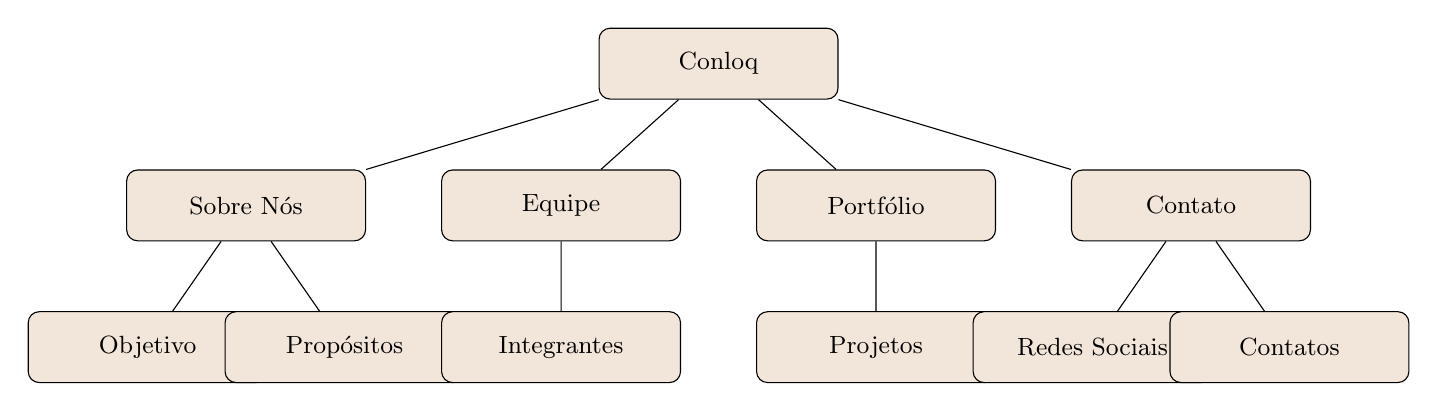
\begin{tikzpicture}[
    level 1/.style={
        sibling distance=4cm,
        level distance=1.8cm
    },
    level 2/.style={
        sibling distance=2.5cm,
        level distance=1.8cm
    },
    every node/.style={
        rectangle,
        draw,
        rounded corners,
        fill=brown!20,
        text width=2.8cm,
        align=center,
        font=\small,
        minimum height=0.9cm
    }
]

\node {Conloq}
    child {
        node {Sobre Nós}
            child { node {Objetivo} }
            child { node {Propósitos} }
    }
    child {
        node {Equipe}
            child { node {Integrantes} }
    }
    child {
        node {Portfólio}
            child { node {Projetos} }
    }
    child {
        node {Contato}
            child { node {Redes Sociais} }
            child { node {Contatos} }
    };
\end{tikzpicture}
\caption{Estrutura de navegação}
\label{fig:sitemap}
\end{figure}

\textbf{Principais seções da landing page da equipe:}

\begin{itemize}

    \item \textbf{Conloq:} Apresentação inicial da equipe e destaque do projeto desenvolvido.

    \item \textbf{Sobre Nós:} Informações sobre a equipe, objetivos e proposta do projeto.

    \item \textbf{Equipe:} Apresentação dos integrantes responsáveis pelo desenvolvimento da plataforma, incluindo nome, função e tecnologias utilizadas.

    \item \textbf{Portfólio:} Exibição dos projetos, tecnologias e soluções desenvolvidas pela equipe.

    \item \textbf{Contato:} Área destinada às informações de comunicação da equipe, contendo links para redes sociais, GitHub, LinkedIn, e-mail e demais canais de contato.

\end{itemize}

\subsection{Especificações Técnicas do Site da Equipe}

\begin{table}[H]
\centering
\caption{Stack Tecnológica}
\label{tab:stack-web}
\begin{tabular}{|l|l|p{6cm}|}
\hline
\textbf{Camada} & \textbf{Tecnologia} & \textbf{Descrição} \\
\hline
Estrutura & HTML5 & Utilizado para estruturar as páginas da landing page \\
\hline
Estilização & CSS3 & Estilização e organização visual da interface \\
\hline
Interatividade & JavaScript & Funcionalidades e interações da página \\
\hline
Responsividade & CSS & Interface para desktop e dispositivos móveis \\
\hline
Hospedagem & GitHub Pages & Deploy e hospedagem do website \\
\hline
Versionamento & Git e GitHub & Gerenciamento e versionamento do código-fonte \\
\hline
\end{tabular}
\end{table}